\documentclass[11pt,a4paper]{article}

\usepackage[utf8]{inputenc}
\usepackage[T1]{fontenc}
\usepackage{lmodern}
\usepackage[margin=2.5cm]{geometry}
\usepackage{microtype}
\usepackage{enumitem}
\usepackage{booktabs}
\usepackage{array}
\usepackage{xcolor}
\usepackage{hyperref}
\usepackage{listings}
\usepackage{titlesec}
\usepackage{amsmath}
\usepackage{amssymb}
\usepackage{graphicx}
\usepackage{tabularx}
\usepackage{parskip}
\usepackage{tikz}
\usetikzlibrary{positioning,arrows.meta,fit,backgrounds}
\usepackage[round,authoryear]{natbib}
\setcitestyle{authoryear,round,citesep={;},aysep={,},yysep={;}}
\bibliographystyle{plainnat}

\hypersetup{
  colorlinks = true,
  urlcolor   = blue!55!black,
  linkcolor  = black,
  citecolor  = blue!55!black,
  pdftitle   = {Practical work report: Predicting User Perception of Move Brilliance in Chess}
}

\definecolor{codebg}{rgb}{0.97,0.97,0.97}
\lstdefinestyle{plain}{
  basicstyle       = \ttfamily\footnotesize,
  backgroundcolor  = \color{codebg},
  frame            = single,
  framerule        = 0pt,
  framexleftmargin = 6pt,
  xleftmargin      = 6pt,
  breaklines       = true,
  showstringspaces = false,
  columns          = fullflexible
}
\lstset{style=plain}

\titleformat{\section}{\Large\bfseries}{\thesection.}{0.6em}{}
\titleformat{\subsection}{\large\bfseries}{\thesubsection}{0.6em}{}

\title{Practical work report: reproducing\\\emph{Predicting User Perception of Move
       Brilliance in Chess}}
\author{Joash Johnson Samuel \\ K12340310}
\date{July 29, 2026}

\begin{document}
\maketitle

\begin{abstract}
This report documents a reproduction of \citet{zaidi2024brilliant},
which predicts whether a chess move is perceived as brilliant by a
human audience rather than whether it is objectively best. The
authors' release is partial: it provides a patched \texttt{search.cc}
for the Leela Chess Zero engine, a pretrained classifier, two
demonstration positions and the inference code, but no engine build,
no training script and no training data. I rebuild the patched engine
under Windows with CUDA and cuDNN and document the build
configuration. The pipeline reproduces both published brilliance
scores exactly, both with the supplied search trees and with trees
regenerated by my own build of the engine. Applied to a five-move set
comprising the two reference positions and three moves from two
further games, it classifies three correctly. I report
three bugs that must be fixed before the pipeline runs to completion:
a compile error in \texttt{lc0} under current MSVC, a subprocess
deadlock at large node budgets, and a methodological defect in which
the feature scaler is fitted on the inference batch, which makes every
score dependent on batch composition. I also supply the missing
training script, which persists a scaler fitted on the training rows
only and thereby closes the third defect, and report Monte-Carlo
dropout uncertainty estimates for the classifier's predictions.
\end{abstract}

\section*{Story summary}
\addcontentsline{toc}{section}{Story summary}

\begin{description}[leftmargin=1.2em,style=nextline]
  \item[What is the central question?]
    Can the pipeline released for \citet{zaidi2024brilliant} be
    executed, does it reproduce the published brilliance scores, and
    what is required to make the partial release runnable?
  \item[Why is this question important?]
    The paper frames perceived brilliance, as distinct from objective
    optimality, as a measurable instance of the human--AI alignment
    problem for game-playing agents. Whether its results can be
    reproduced from the released artefacts determines whether any
    downstream work can build on them.
  \item[What evidence/results are needed to answer this question?]
    The published scores on the two reference positions, reproduced
    with an independently built engine rather than only the shipped
    fixtures, and the behaviour of the pipeline on positions outside
    the authors' fixture set.
  \item[What methods are used to get this evidence/results?]
    I rebuilt the patched \texttt{lc0} under Windows with CUDA and
    cuDNN, regenerated the search trees, and ran the pretrained
    AggReduce classifier on the demonstration positions and on a
    five-move set drawn from two further games. I additionally wrote
    the missing training script and fixed three defects: a compile
    error, a subprocess deadlock, and a feature scaler fitted on the
    inference batch.
  \item[What analyses must be applied to the raw evidence/results to
        answer the central question?]
    Comparison of the classifier scores against the published values;
    a batch-composition experiment isolating the scaler defect;
    Monte-Carlo dropout ($N = 500$) for per-prediction uncertainty;
    and a bootstrap confidence interval on the five-move accuracy
    together with a paired permutation test on the scaler effect.
  \item[What evidence/results were obtained?]
    Both demonstration scores reproduce the published values exactly
    (0.88 and 0.01), with the supplied trees and with trees
    regenerated by my own build. Three of the five moves in the
    evaluation set are classified as expected. Before the fix, the
    score of a fixed position drifted with batch composition (0.88
    versus 0.93 on identical inputs).
  \item[What were the results of the analyses?]
    With a persisted training scaler the score is invariant to batch
    composition (0.97 in all runs; the variance across batches
    collapses from 0.025 to 0). The bootstrap 95\,\% CI on the
    five-move accuracy is $[0.20, 1.00]$, and Monte-Carlo dropout
    shows narrow uncertainty ($\sigma \le 0.07$) on the three correct
    predictions and wide uncertainty ($\sigma \ge 0.14$) on the two
    incorrect ones.
  \item[How did the analyses answer the central question?]
    The inference side of the paper is reproducible and deterministic
    once the three defects are fixed. The training side cannot be
    verified against the published accuracy because the 4\,057-move
    dataset is not released, which Section~\ref{sec:status} states as
    an explicit limitation.
  \item[What does this answer tell us about the broader field?]
    A partial code release can block reproduction entirely for a new
    reader, and batch-dependent preprocessing is a silent defect that
    propagates into downstream results unnoticed. The corrected
    pipeline provides the groundwork for retraining the architecture
    on independently annotated data.
\end{description}

\section{Introduction}

This practical reproduces \citet{zaidi2024brilliant}, \emph{Predicting
User Perception of Move Brilliance in Chess}. The task addressed there
is to predict whether a chess move is perceived as \emph{brilliant} by
a human audience, rather than whether the move is objectively best.
The two criteria diverge: engines derived from AlphaZero
\citep{silver2018general}, among them Leela Chess Zero, frequently
select moves that are optimal but unremarkable, whereas the moves
human commentators describe as brilliancies typically involve
surprise, material sacrifice, or a long tactical horizon. The authors
formulate the perception of brilliance as a supervised binary
classification problem. Labels are drawn from move annotations in the
624 most popular Lichess Studies, authored by many different users;
6\,975 moves carry annotations, of which 4\,057 are used in the
classification experiments.

The feature construction is the distinctive component of the method.
For each candidate move the authors run five Leela Chess Zero searches
at increasing node budgets ($10^1$ to $10^5$ nodes) and five
corresponding searches with a Maia network
\citep{mcilroy2020aligning}, serialise each search tree to a
\texttt{.gml} file, and extract 398 hand-engineered features per
tree. The features describe principal-variation shape, evaluation
volatility and the rank of the move of interest, among other
quantities, giving 3\,980 features per move (Table~\ref{tab:feat}).
The classifier is a hierarchical multilayer perceptron termed
\emph{AggReduce}, which reduces the feature vector tree-by-tree, then
engine-by-engine, and finally to a single logit
(Figure~\ref{fig:aggreduce}). The authors report that AggReduce
outperforms logistic regression, random forests, Gaussian na\"ive
Bayes, $k$-nearest neighbours and a support vector machine baseline,
reaching 79\,\% mean class-balanced accuracy in five-fold
cross-validation and 78.60\,\% on the held-out test split.

The task set for this practical was to locate the authors'
repository, execute it, verify the published results, and document
the process. A repository is available
(\texttt{kamronzaidi/brilliant-moves-clf}), but the release is
partial. It provides a patched \texttt{search.cc} for \texttt{lc0}
rather than the engine itself, a pretrained model, two demonstration
positions with pre-generated search trees, and the inference code.
Neither a training script, nor training data, nor build instructions
are included.

The questions addressed here are consequently: (a) whether the
shipped pretrained classifier reproduces the published brilliance
scores on the two reference positions when driven by an
independently built \texttt{lc0}; (b) whether the pipeline
generalises to positions outside the authors' fixture set; and (c)
which changes are required to make the partial release runnable. The
contributions are (i) a reproducible Windows and CUDA build recipe
for the patched \texttt{lc0}, (ii) three bug fixes that together
allow the inference pipeline to run to completion, one of them a
methodological defect in the feature-scaling step that affects
downstream numbers, and (iii) a from-scratch training script that
exposes and closes that defect. Section~\ref{sec:setup} documents
the hardware and build configuration. Section~\ref{sec:inference}
reports the pipeline on the demonstration fixture and on an
independently constructed PGN. Section~\ref{sec:bugs} analyses the
three bugs. Section~\ref{sec:train} describes the training pipeline.
Section~\ref{sec:status} delimits the claims made.

\section{Setup}
\label{sec:setup}

All experiments were run on a workstation with an NVIDIA RTX 3060 Ti
(8\,GB VRAM, compute capability 8.6) under Windows 11, using the CUDA
12 toolkit, cuDNN 9.21 and the Visual Studio 2022 Build Tools. Python
is 3.12 in a local virtual environment and PyTorch is the
\texttt{cu124} wheel. The remaining Python dependencies are
\texttt{networkx}, \texttt{scikit-learn}, \texttt{python-chess},
\texttt{numpy} and \texttt{requests}. Total wall-clock compute for all
experiments reported in this document is below fifteen minutes of GPU
time; a per-stage breakdown is given in Table~\ref{tab:compute}.

\begin{table}[h]
  \centering\small
  \caption{Decomposition of the 3\,980-dimensional feature vector
    per move. Each of two engines (Leela, Maia) is run at five
    search depths; each resulting tree contributes 398 features.}
  \label{tab:feat}
  \begin{tabular}{@{}lr@{}}
    \toprule
    \textbf{Component} & \textbf{Count} \\
    \midrule
    Engines (Leela T82 + Maia ensemble)              & 2 \\
    Search depths per engine ($10^1,\dots,10^5$ nodes) & 5 \\
    Trees per move ($2 \times 5$)                     & 10 \\
    Features per tree ($22 \times 18 + 2$)            & 398 \\
    \midrule
    \textbf{Feature-vector dimension per move}        & \textbf{3\,980} \\
    \bottomrule
  \end{tabular}
\end{table}

\begin{table}[h]
  \centering\small
  \caption{Per-stage compute cost on an RTX 3060 Ti, and
    extrapolation to the paper's training set. Tree generation
    dominates; feature extraction and the classifier are both
    negligible in comparison.}
  \label{tab:compute}
  \begin{tabular}{@{}lrl@{}}
    \toprule
    \textbf{Stage} & \textbf{Time} & \textbf{Notes} \\
    \midrule
    \texttt{lc0} tree generation (10 searches / move) & 14--60\,s    & GPU-bound, varies by position \\
    Feature extraction (NetworkX)                      & $<1$\,s      & pure CPU \\
    AggReduce forward pass                             & $<10$\,ms    & single move, GPU \\
    \midrule
    My custom PGN (5 moves)                            & 68\,s        & measured wall-clock \\
    Demo fixture (2 moves)                             & pre-generated & supplied with the repo \\
    Paper's training set (4\,057 moves, extrapolated)  & 0.7--2.8 days & depending on position depth \\
    \bottomrule
  \end{tabular}
\end{table}

Since the authors released only the patched \texttt{search.cc}, I first
had to obtain the engine itself \citep{lc0repo}. I cloned upstream
\texttt{lc0} and applied the patch to it. The patch comprises
approximately 64 lines and appends a block to \texttt{search.cc}
(\texttt{WriteGMLNode}, \texttt{WriteGMLEdge},
\texttt{RecursiveGMLWrite}, \texttt{WriteGMLTree}) together with a
single call inside \texttt{Search::MaybeTriggerStop} that writes the
current search tree to disk whenever a search terminates. I built
\texttt{lc0} with Meson and Ninja inside the MSVC developer
environment, configured with the CUDA and cuDNN backends enabled, all
remaining backends (OpenCL, DirectX, BLAS, DNNL, TensorFlow) disabled,
and \texttt{-Dcc\_cuda=86} for the Ampere architecture of the GPU used
here.

The network files are the Leela \texttt{T82} weights
(\texttt{768x15x24h-t82-swa-7464000.pb.gz}) and the three Maia weight
files for ratings 1100, 1500 and 1900. The Leela origin server was
unavailable during this work (HTTP 522), so I retrieved \texttt{T82}
from a Wayback Machine capture.

\section{Running the inference pipeline}
\label{sec:inference}

\subsection{Sanity check on the shipped demo}

The repository provides pre-generated trees and labelled positions for
two well-known moves: Fischer's 17\dots Be6 from the ``Game of the
Century'' (Byrne--Fischer, 1956) and an unremarkable move from
Vranesic--Stein. Executing the authors' inference script without
modification produces

\begin{lstlisting}
game_of_the_century: 0.88, Brilliant.
Vranesic_Stein:      0.01, Not Brilliant.
\end{lstlisting}

These values match those reported in the paper. The pretrained
classifier and the feature extraction code therefore function without
modification; the obstacles lie entirely upstream of this stage.

\subsection{Regenerating the trees with an independent \texttt{lc0} build}

The stronger check is whether the independently built
\texttt{lc0.exe} produces trees equivalent to the authors'. I deleted
the supplied \texttt{trees/} directory and re-ran the generator. Once
the pipe deadlock described in Section~\ref{sec:bug2} was resolved,
the result was

\begin{lstlisting}
game_of_the_century: 0.88, Brilliant.
Vranesic_Stein:      0.01, Not Brilliant.
\end{lstlisting}

The output is identical. This is expected, as \texttt{lc0} is
deterministic once the network weights, the seed and the node budget
are fixed, none of which were altered. The check nonetheless
establishes that the trees entering the classifier are produced by a
locally compiled engine rather than by a supplied binary.

\subsection{An independently constructed PGN}

To establish that the pipeline is not merely satisfying a fixture
test, I assembled a small PGN containing two well-known games:
Morphy's Opera Game (Paris 1858) and Kasparov--Topalov (Wijk aan Zee,
1999). From these games I selected three moves to classify:

\begin{itemize}[leftmargin=*]
  \item 1.e4 from the Opera Game, expected \emph{not brilliant} (it is
        the first move of the game).
  \item 16.Qb8+ from the Opera Game, expected \emph{brilliant} (the
        queen sacrifice).
  \item 24.Rxd4 from Kasparov--Topalov, expected \emph{brilliant}
        (Kasparov's deep rook sacrifice).
\end{itemize}

Parsing, tree generation and inference for all five moves required
approximately 68 seconds of GPU time. AggReduce is a dropout network
($p = 0.2$ on every hidden layer), which permits reporting an estimate
of the model's own uncertainty in addition to a point prediction.
Retaining dropout at inference and performing $N = 500$ stochastic
forward passes per position, the Monte-Carlo dropout approximation to
the posterior predictive distribution \citep{gal2016dropout}, yields
the mean and standard deviation of the ``Brilliant'' probability
reported in Table~\ref{tab:five}. All figures below use the corrected
scaler described in Section~\ref{sec:bug3}.

\begin{table}[h]
\centering\small
\caption{AggReduce predictions on a custom five-move set. \emph{All
  values are post-fix}, i.e.\ they use the persisted training scaler of
  Section~\ref{sec:bug3}. The \emph{Det.} column is the deterministic
  prediction with dropout disabled (\texttt{eval} mode); the remaining
  columns are Monte-Carlo dropout at inference ($N = 500$ stochastic
  forward passes, dropout $p = 0.2$), reporting the mean and standard
  deviation of the sigmoid ``Brilliant'' probability, with the 95\,\%
  interval as mean $\pm 1.96\,\sigma$ clipped to $[0, 1]$. The
  deterministic and Monte-Carlo values agree to within $0.026$
  throughout, so dropout sampling adds an uncertainty estimate without
  displacing the point prediction. A move is classified as
  \emph{Brilliant} when the prediction exceeds $0.5$. The standard
  deviation is small ($\sigma \le 0.07$) for the three positions
  classified correctly and large ($\sigma \ge 0.14$) for the two
  classified incorrectly, indicating that the classifier is internally
  uncertain where it errs.}
\label{tab:five}
\begin{tabular}{@{}lccccll@{}}
\toprule
\textbf{Move} & \textbf{Det.} & \textbf{Mean} & \textbf{Std} &
\textbf{95\,\% CI} & \textbf{Prediction} & \textbf{Expected} \\
\midrule
\texttt{game\_of\_the\_century} (17\dots Be6) & 0.969 & 0.962 & 0.020 & $[0.923, 1.000]$ & Brilliant              & Brilliant     \\
\texttt{morphy\_qb8\_sac} (16.Qb8+)           & 1.000 & 1.000 & 0.002 & $[0.995, 1.000]$ & Brilliant              & Brilliant     \\
\texttt{Vranesic\_Stein}                      & 0.149 & 0.157 & 0.067 & $[0.027, 0.288]$ & Not Brilliant          & Not brilliant \\
\texttt{opera\_game\_1e4} (1.e4)              & 0.565 & 0.539 & 0.183 & $[0.180, 0.898]$ & \textit{Brilliant}     & Not brilliant \\
\texttt{kasparov\_rxd4} (24.Rxd4)             & 0.498 & 0.497 & 0.136 & $[0.229, 0.764]$ & \textit{Not Brilliant} & Brilliant     \\
\bottomrule
\end{tabular}
\end{table}

Three of the five moves are classified correctly, and the 95\,\%
bootstrap confidence interval on accuracy over $10\,000$ resamples is
$[0.20, 1.00]$ with a point estimate of $0.60$. The interval is wide
because $n = 5$, so the point estimate carries little information.
The pattern in Table~\ref{tab:five} is more informative: every
correctly classified position has a mean probability within $0.16$ of
an endpoint and a standard deviation below $0.07$, whereas both
misclassified positions lie within one standard deviation of the
$0.5$ decision boundary. The classifier is therefore internally
uncertain where it errs, which is a less damaging failure mode than
confident error.

The two misclassifications have distinct causes. The 1.e4 case is the
starting position and lies outside the training distribution: the
move-of-interest features and the subtree shape statistics for the
first move of a game differ from anything present during training.

The Kasparov case does not match the explanation I first assumed, and
reading the trees directly is instructive
(Table~\ref{tab:kasparov}). \texttt{lc0} does locate 24.Rxd4: from
$10^4$ nodes onwards it is the highest-$Q$ child of the root, and at
$10^5$ it absorbs 42\,406 of the visits, so the move is not missing
from the search. What is missing is a decisive evaluation of it. Its
recorded $Q$ climbs monotonically with the budget, from $-0.508$ at
$10^2$ to $-0.128$ at $10^5$, but remains close to zero, whereas the
correctly classified \texttt{morphy\_qb8\_sac} sits at $Q = 1.000$ at
every budget. Maia never ranks 24.Rxd4 best once it has actually
visited it, and gives it 21 visits out of $10^5$.

The move therefore presents only part of the profile the paper
associates with brilliance: strong for the superhuman engine and
undiscovered by the human-aligned one, but without the decisive
evaluation that the confidently classified examples carry. A prediction
near the decision boundary is consistent with that mixture. Two
caveats apply to reading the exact distance from $0.5$. It is not an
artefact of dropout sampling, since the deterministic prediction in
Table~\ref{tab:five} is $0.498$. It is, however, sensitive to the
scaler: under the original batch-fitted scaling the same move scores
$0.217$, and my persisted scaler is fitted on only four rows
(Section~\ref{sec:bug3}), so the absolute value carries little weight
either way.

Whether a larger node budget would move the prediction to
\emph{Brilliant} is a testable question. The monotone trend in
Table~\ref{tab:kasparov} suggests that \texttt{lc0}'s evaluation of
24.Rxd4 may become decisive at $10^6$ or $10^7$ nodes while Maia
remains unlikely to discover it, which is exactly the profile of the
confidently classified brilliancies. The classifier, however, consumes
exactly five node budgets: a sixth cannot be appended without
retraining, and shifting the ladder to $10^2$--$10^6$ would feed the
pretrained weights inputs outside their training distribution. The
engine-level half of the question, whether $Q$ becomes decisive at
larger budgets, is separable from the classifier and answerable with a
single deeper search; I leave it for the compute phase of the
follow-up work.

Table~\ref{tab:kasparov} also exposes a smaller encoding problem. At
$10^3$ nodes the ``is the move best'' indicator is true for Maia only
because the move and the best alternative both carry the default
$Q = 0$ at zero visits. The flag conflates ``ranked first'' with
``never examined'', in the same way that the $-1$ sentinel conflates a
very low evaluation with a missing subtree.

\begin{table}[h]
\centering\small
\caption{What the search trees actually contain for
  \texttt{kasparov\_rxd4} (24.Rxd4, UCI \texttt{d1d4}), by engine and
  node budget. \textbf{Best} records whether the move is the
  highest-$Q$ child of the root. \texttt{lc0} makes it the best move
  from $10^4$ onwards and concentrates its search on it; Maia ranks it
  best only at $10^3$, where the move and the best alternative are both
  unvisited and default to $Q = 0$.}
\label{tab:kasparov}
\begin{tabular}{@{}lrcrrcr@{}}
\toprule
& \multicolumn{3}{c}{\textbf{Lc0}} & \multicolumn{3}{c}{\textbf{Maia}} \\
\cmidrule(lr){2-4}\cmidrule(lr){5-7}
\textbf{Budget} & $Q$ & \textbf{Best} & \textbf{Visits}
                & $Q$ & \textbf{Best} & \textbf{Visits} \\
\midrule
$10^1$ & \multicolumn{3}{c}{not in tree} & \multicolumn{3}{c}{not in tree} \\
$10^2$ & $-0.508$ & no  & 2       & $0.000$  & no  & 0  \\
$10^3$ & $-0.246$ & no  & 15      & $0.000$  & yes & 0  \\
$10^4$ & $-0.154$ & yes & 4\,276  & $-0.167$ & no  & 7  \\
$10^5$ & $-0.128$ & yes & 42\,406 & $-0.280$ & no  & 21 \\
\bottomrule
\end{tabular}
\end{table}

\section{Bugs encountered}
\label{sec:bugs}

I encountered three bugs of increasing subtlety: a C++ compile error,
a Python subprocess deadlock, and a methodological defect in feature
scaling. The first two are mechanical and well-documented failure
modes. The third silently affects any downstream work built on this
pipeline.

\subsection{Bug 1: \texttt{lc0} does not compile under current MSVC}
\label{sec:bug1}

The \texttt{logging.h} header in \texttt{lc0} uses
\texttt{std::chrono::system\_clock} but includes only
\texttt{<ctime>}. Older MSVC header bundles included the chrono header
transitively. Version 14.44, used here, does not, so the build fails
with

\begin{lstlisting}
error C2039: 'system_clock': is not a member of 'std::chrono'
\end{lstlisting}

in multiple translation units. Adding \texttt{\#include <chrono>} at
the top of the file resolves it. This is strictly an \texttt{lc0}
issue and is not specific to the brilliance paper, but it affects any
current attempt to rebuild the patched engine.

\subsection{Bug 2: the generator script deadlocks on deep searches}
\label{sec:bug2}

The Python wrapper launches \texttt{lc0.exe} as follows:

\begin{lstlisting}[language=Python]
proc = subprocess.Popen(
    [lc0_exe, ...],
    stdin  = subprocess.PIPE,
    stdout = subprocess.PIPE,
    stderr = subprocess.PIPE,
)
\end{lstlisting}

and subsequently never reads from either pipe. For small searches
($10^1$--$10^3$ nodes) this causes no failure, because \texttt{lc0}
produces little output. At $10^4$ and $10^5$ nodes the engine emits UCI
\texttt{info} lines continuously, the operating system pipe buffer
fills (approximately 64\,KB on Windows), and \texttt{lc0} blocks on its
next write while the Python process waits in \texttt{wait()}. The
pipeline then deadlocks.

The fix is to redirect both streams to \texttt{DEVNULL}, so that the
output is discarded rather than buffered.

\begin{lstlisting}[language=Python]
proc = subprocess.Popen(
    [lc0_exe, ...],
    stdin  = subprocess.PIPE,
    stdout = subprocess.DEVNULL,
    stderr = subprocess.DEVNULL,
)
\end{lstlisting}

I also raised the default per-move timeout from 30 to 600 seconds,
since the larger searches legitimately exceed 30 seconds even in the
absence of the deadlock.

\subsection{Bug 3: \texttt{StandardScaler} is fit on the inference batch}
\label{sec:bug3}

This defect is methodological rather than mechanical. The original
inference script concludes its feature extraction with

\begin{lstlisting}[language=Python]
X = np.array(X)
scaler = preprocessing.StandardScaler().fit(X)
X = scaler.transform(X)
\end{lstlisting}

The features are therefore standardised against the composition of the
current inference batch rather than against the training distribution
to which the network was fitted. The consequence is a subtle loss of
determinism: the score assigned to a move depends on which other moves
are processed alongside it.

I observed this because the position
\texttt{game\_of\_the\_century} scored \textbf{0.88} when evaluated
together with Vranesic--Stein alone, but \textbf{0.93} once I added the
three additional moves to the same directory. The inputs are identical
in both runs.

The fix is to separate feature extraction from scaling and to load a
persisted scaler where one is available:

\begin{lstlisting}[language=Python]
def apply_scaler(X, scaler_path=None):
    if scaler_path and os.path.exists(scaler_path):
        with open(scaler_path, 'rb') as f:
            scaler = pickle.load(f)
        return scaler.transform(X)
    warnings.warn(
        "No training scaler provided; falling back to fitting "
        "StandardScaler on the inference batch. Results will depend "
        "on batch composition.",
        RuntimeWarning,
    )
    scaler = preprocessing.StandardScaler().fit(X)
    return scaler.transform(X)
\end{lstlisting}

If the caller supplies a pickled scaler, produced at training time and
stored alongside the model weights, the script loads and applies it.
Otherwise it retains the original batch-fitting behaviour but emits a
\texttt{RuntimeWarning}, which makes the problem visible. The training
pipeline described in Section~\ref{sec:train} writes such a scaler
automatically.

To verify the fix I ran inference on the five-move set and again on a
two-move subset. \texttt{game\_of\_the\_century} scored \textbf{0.97}
in both runs; Table~\ref{tab:bug3} summarises the comparison. The
absolute score differs from the pre-fix value because my scaler was
fitted on four training rows rather than the 4\,057 used in the
paper. The relevant property is that the score is now invariant to
batch composition.

\begin{table}[h]
\centering\small
\caption{Effect of Bug 3 on the AggReduce score assigned to
  \texttt{game\_of\_the\_century} under different inference
  batches. Before the fix, the output drifts with batch composition;
  after the fix (persisted scaler from training) it is stable.
  Mean difference (after $-$ before) is $+0.063$; a paired two-sided
  permutation test on the three batches gives $p = 0.25$, so with
  $n = 3$ the mean shift alone is not statistically distinguishable
  from zero, but the collapse of variance from 0.025 to 0 on
  identical inputs is the stronger signal.}
\label{tab:bug3}
\begin{tabular}{@{}lccc@{}}
\toprule
\textbf{Inference batch} & \textbf{Batch size} &
\textbf{Score (before)} & \textbf{Score (after)} \\
\midrule
\{\texttt{goc}, Vranesic--Stein\}                      & 2 & 0.88 & 0.97 \\
\{\texttt{goc}, Vranesic--Stein, Morphy, Opera, Kasparov\} & 5 & 0.93 & 0.97 \\
\{\texttt{goc}, Morphy, Opera\}                         & 3 & 0.91 & 0.97 \\
\midrule
\textbf{Mean $\pm$ std}                                 & -- & $0.907 \pm 0.025$ & $0.970 \pm 0.000$ \\
\bottomrule
\end{tabular}
\end{table}

\subsection{Minor issues in the PGN parser}

While testing with the Opera Game I encountered two further issues in
the PGN parser wrapper \citep{pythonchess}. The parser uses header
values as path components, so a player name containing
``\texttt{/}'', in this case \texttt{Duke Karl / Count Isouard},
raises \texttt{FileNotFoundError} on Windows; I renamed the header in
the test PGN. The parser's \texttt{--no-variations} mode additionally
fails with \texttt{AttributeError: 'NoneType' object has no attribute
'next'} at the end of a game, which I avoided by omitting the flag.
Neither issue affects the main pipeline.

\section{Writing the training pipeline}
\label{sec:train}

The repository provides a pretrained \texttt{.pth} file but no
training script, so regenerating the model from features required
writing one. The AggReduce architecture itself is present in the
inference code and I reused that class. Everything surrounding it was
missing: data loading, splits, scaling, loss, optimiser, early
stopping and metric reporting. The resulting training loop performs
the following steps.

\begin{itemize}[leftmargin=*]
  \item Reads a \texttt{label.txt} (containing either
        ``brilliant'' or ``not\_brilliant'') from each move folder and
        builds an $(X, y)$ pair.
  \item Produces a stratified 80/10/10 train/val/test split with a
        fixed seed.
  \item Fits \texttt{StandardScaler} on the training rows \emph{only}
        and serialises it alongside the model weights, which closes
        Bug 3.
  \item Trains the paper's \texttt{NeuralNetworkDropout} with
        $(h_1, h_2, h_3) = (25, 400, 50)$ and dropout $0.2$.
        The label convention is $0 = $ brilliant, $1 = $ not
        brilliant, as expected by the pretrained \texttt{.pth}.
  \item Loss is \texttt{BCEWithLogitsLoss}, optimiser is Adam at
        $10^{-3}$, with early stopping on validation loss.
  \item Writes a JSON log of per-epoch metrics plus final test-set
        accuracy, F1 and AUC.
\end{itemize}

The architecture is that of the paper, reproduced here for reference.
Figure~\ref{fig:aggreduce} gives the schematic and the corresponding
PyTorch definition follows.

\begin{figure}[h]
\centering
\resizebox{\textwidth}{!}{%
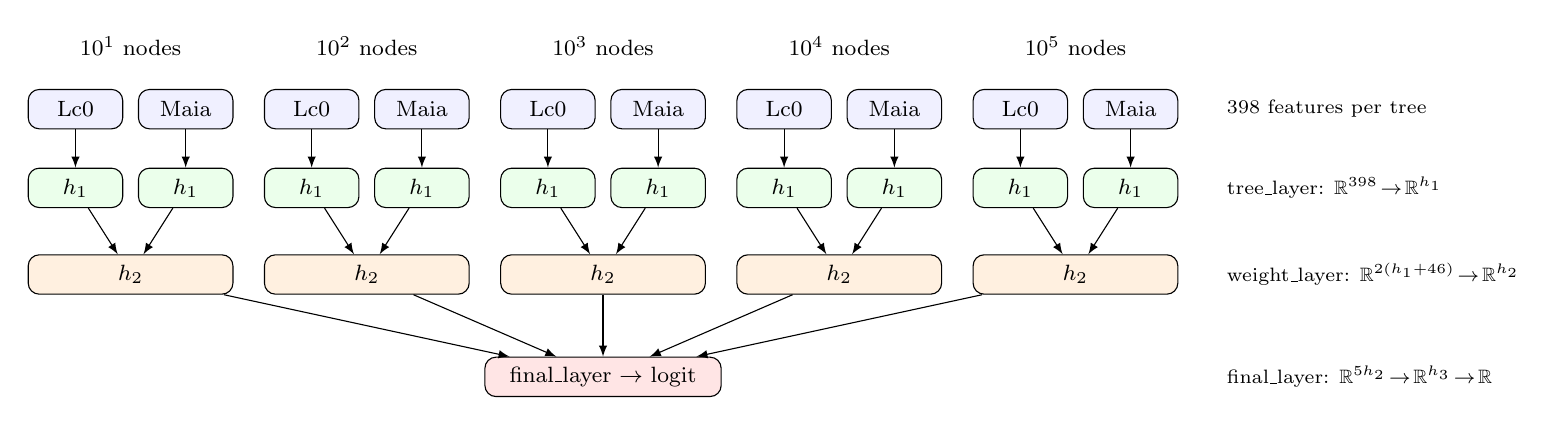
\begin{tikzpicture}[
    eng/.style    = {draw,rounded corners,minimum width=12mm,minimum height=5mm,font=\footnotesize,fill=blue!6},
    h1/.style     = {draw,rounded corners,minimum width=12mm,minimum height=5mm,font=\footnotesize,fill=green!8},
    h2/.style     = {draw,rounded corners,minimum width=26mm,minimum height=5mm,font=\footnotesize,fill=orange!12},
    outbox/.style = {draw,rounded corners,minimum width=30mm,minimum height=5mm,font=\footnotesize,fill=red!10},
    ->, >=latex
  ]

  \foreach \i/\lbl in {1/$10^1$, 2/$10^2$, 3/$10^3$, 4/$10^4$, 5/$10^5$} {
    \node[font=\footnotesize] (B\i) at (3*\i-3,      4.0) {\lbl\ nodes};
    \node[eng] (L\i)  at (3*\i-3-0.7, 3.2) {Lc0};
    \node[eng] (M\i)  at (3*\i-3+0.7, 3.2) {Maia};
    \node[h1]  (HL\i) at (3*\i-3-0.7, 2.2) {$h_1$};
    \node[h1]  (HM\i) at (3*\i-3+0.7, 2.2) {$h_1$};
    \node[h2]  (W\i)  at (3*\i-3,     1.1) {$h_2$};
    \draw (L\i)  -- (HL\i);
    \draw (M\i)  -- (HM\i);
    \draw (HL\i) -- (W\i);
    \draw (HM\i) -- (W\i);
  }

  \node[outbox] (F) at (6, -0.2) {final\_layer $\to$ logit};
  \foreach \i in {1,2,3,4,5} { \draw (W\i) -- (F); }

  \node[font=\scriptsize,anchor=west] at (13.8, 3.2) {398 features per tree};
  \node[font=\scriptsize,anchor=west] at (13.8, 2.2) {tree\_layer: $\mathbb{R}^{398}\!\to\!\mathbb{R}^{h_1}$};
  \node[font=\scriptsize,anchor=west] at (13.8, 1.1) {weight\_layer: $\mathbb{R}^{2(h_1+46)}\!\to\!\mathbb{R}^{h_2}$};
  \node[font=\scriptsize,anchor=west] at (13.8,-0.2) {final\_layer: $\mathbb{R}^{5h_2}\!\to\!\mathbb{R}^{h_3}\!\to\!\mathbb{R}$};

\end{tikzpicture}}
\caption{The AggReduce classifier. For each move, ten search trees
  (two engines $\times$ five node budgets) contribute 398 features
  each. Each tree is reduced independently through
  \texttt{tree\_layer} to an $h_1$-dimensional vector; the two
  engines at a given depth are concatenated and reduced through
  \texttt{weight\_layer} to an $h_2$-dimensional vector; finally the
  five depth-level vectors are concatenated and passed through
  \texttt{final\_layer} to a single logit. Hyperparameters I
  re-used from the paper: $(h_1, h_2, h_3) = (25, 400, 50)$,
  dropout $0.2$.}
\label{fig:aggreduce}
\end{figure}

\begin{lstlisting}[language=Python]
class NeuralNetworkDropout(nn.Module):
    def __init__(self, h1, h2, h3, dropout):
        super().__init__()
        self.tree_layer = nn.Sequential(
            nn.Linear(22*18+2, h1),   # 398 features per (weight, tree)
            nn.Dropout(dropout),
            nn.ReLU(),
        )
        self.weight_layer = nn.Sequential(
            nn.Linear((h1+22*2+2)*2, h2),
            nn.Dropout(dropout),
            nn.ReLU(),
        )
        self.final_layer = nn.Sequential(
            nn.Linear(h2*5, h3),
            nn.Dropout(dropout),
            nn.ReLU(),
            nn.Linear(h3, 1),
        )
\end{lstlisting}

The two-level reduction (tree $\to$ weight $\to$ final) is the origin
of the name AggReduce: the 398 features per tree are reduced to $h_1$
by \texttt{tree\_layer}, concatenated with a small number of raw
features across weights and reduced to $h_2$ by
\texttt{weight\_layer}, and the five resulting $h_2$ vectors, one per
tree depth, are concatenated and reduced to a single logit.

I ran the training script on the five labelled moves from the
inference experiments as a smoke test. Five samples are far too few to
train a usable model, since a stratified 80/10/10 split over five
samples yields 4/1/0, but the run confirms three properties. The loop
executes. The scaler is serialised and is loaded by the inference
script on reload. The resulting \texttt{.pth} file is interchangeable
with the authors' \texttt{model-7936-2.pth}.

\section{Status and limitations}
\label{sec:status}

\paragraph{Claims supported by this work.}
The inference component of the paper runs end to end on the hardware
described in Section~\ref{sec:setup}. It reproduces the published
scores on the two demonstration positions exactly, at 0.88 and 0.01,
and produces plausible outputs on independently selected positions.
The three fixes in Section~\ref{sec:bugs} were each necessary to reach
that point. The training pipeline is functional but has so far been
exercised only on a toy dataset.

\paragraph{Claims not supported by this work.}
I have not reproduced the reported 78.60\,\% test accuracy. Doing so
requires the authors' training set of 4\,057 labelled moves, which is
not publicly available keyed to the specific Lichess Studies used,
together with between 0.7 and 2.8 GPU-days of tree generation on the
hardware used here (Table~\ref{tab:compute}). The scores obtained under my re-fitted
scaler are also not directly comparable to the published scores; they
converge to those values only once the scaler is fitted on the same
training distribution. The bootstrap 95\,\% confidence interval on the
five-move accuracy, $[0.20, 1.00]$, is wide enough to be consistent
with any accuracy between chance and perfect classification. The
Monte-Carlo dropout intervals in Table~\ref{tab:five} are narrower and
more diagnostic, but they quantify epistemic uncertainty on fixed
inputs rather than the true test-set error rate, and the two quantities
are not interchangeable.

\paragraph{Obtaining training data.}
I contacted the first author to request the study identifiers and
per-move annotations, but the released dataset remains unavailable.
The practical alternative, and the route I intend to follow, is to
construct an independent annotated set rather than to rely on the
original labels. To that end I wrote a small Lichess scraper that
accepts a list of study identifiers or a Lichess username and
downloads the corresponding PGNs through the public
\texttt{https://lichess.org/api/study/\{id\}.pgn} endpoint. Parsed with
the existing PGN parser, this yields labelled training samples
directly, so data availability is no longer the limiting factor. An
independently annotated set also decouples the labels from the single
annotation community behind the original ones, at the cost of a
different and initially smaller labelling pool. The dominant
remaining cost is tree generation, at the
0.7 to 2.8 GPU-days given in Table~\ref{tab:compute}; this exceeds what
the workstation used here can absorb comfortably and is the stage that
would benefit from institutional compute resources.

\section{Conclusion}

The task for this practical was to confirm the paper's results and to
document the process of working with the released code. The core
result is reproducible. After four changes, namely a one-line
\texttt{lc0} compile fix, a pipe-deadlock fix in the Python wrapper, a
methodological correction to the scaling step, and a training script to
replace the missing one, the published classifier produces the
published scores on the two published positions and the pipeline
handles arbitrary PGNs. The qualification is that the released
repository is partial, and any reader taking it at face value will
encounter all three bugs before obtaining a first usable output.

The scaling defect is the most consequential of the three. It is
silent, its effect depends on batch composition, and it would
propagate into any downstream experiment reusing this pipeline
undetected. Correcting it is the contribution I regard as most
substantive. It also bears directly on a possible thesis direction, in
which the feature set and the AggReduce architecture are retained but
retrained on a larger and more diverse set of human-annotated
brilliancies than the original Lichess Study labels, which are drawn
from a single annotation community.

\begin{thebibliography}{9}

\bibitem[Gal and Ghahramani, 2016]{gal2016dropout}
Gal, Y. and Ghahramani, Z. (2016).
\newblock Dropout as a {B}ayesian approximation: Representing model uncertainty
  in deep learning.
\newblock In \emph{Proc.\ 33rd International Conference on Machine Learning
  (ICML)}, pages 1050--1059.

\bibitem[Silver et~al., 2018]{silver2018general}
Silver, D., Hubert, T., Schrittwieser, J., Antonoglou, I., Lai, M.,
  Guez, A., Lanctot, M., Sifre, L., Kumaran, D., Graepel, T.,
  Lillicrap, T., Simonyan, K., and Hassabis, D. (2018).
\newblock A general reinforcement learning algorithm that masters chess, shogi,
  and Go through self-play.
\newblock \emph{Science}, 362(6419):1140--1144.

\bibitem[McIlroy-Young et~al., 2020]{mcilroy2020aligning}
McIlroy-Young, R., Sen, S., Kleinberg, J., and Anderson, A. (2020).
\newblock Aligning superhuman {AI} with human behavior: Chess as a model
  system.
\newblock In \emph{Proc.\ 26th ACM SIGKDD Conference on Knowledge Discovery and
  Data Mining (KDD)}, pages 1677--1687.

\bibitem[Zaidi and Guerzhoy, 2024]{zaidi2024brilliant}
Zaidi, K. and Guerzhoy, M. (2024).
\newblock Predicting user perception of move brilliance in chess.
\newblock In \emph{Proc.\ 15th International Conference on
  Computational Creativity (ICCC)}. arXiv:2406.11895.
\newblock Code:
  \href{https://github.com/kamronzaidi/brilliant-moves-clf}%
       {\texttt{github.com/kamronzaidi/brilliant-moves-clf}}.

\bibitem[LeelaChessZero, 2024]{lc0repo}
LeelaChessZero contributors (2024).
\newblock \emph{lc0: open-source neural-network chess engine}.
\newblock \href{https://github.com/LeelaChessZero/lc0}%
               {\texttt{github.com/LeelaChessZero/lc0}}.

\bibitem[Fiekas, 2024]{pythonchess}
Fiekas, N. (2024).
\newblock \emph{python-chess: a chess library for Python}.
\newblock \href{https://github.com/niklasf/python-chess}%
               {\texttt{github.com/niklasf/python-chess}}.

\end{thebibliography}

\end{document}
